\documentclass[10pt]{article}
\usepackage[a4paper,margin=1.9cm,top=1.6cm,bottom=1.6cm]{geometry}
\usepackage[T1]{fontenc}
\usepackage{newtxtext,newtxmath}
\usepackage{microtype}
\usepackage{graphicx,booktabs,amsmath,enumitem,array}
\usepackage[font=small,labelfont=bf]{caption}
\usepackage[hidelinks]{hyperref}
\usepackage{titlesec}
\titleformat{\section}{\normalfont\fontsize{11}{13}\bfseries}{\thesection}{0.6em}{}
\titlespacing*{\section}{0pt}{8pt}{3pt}
\setlist{nosep,leftmargin=1.4em,topsep=2pt,itemsep=1pt}
\setlength{\parskip}{3pt}\setlength{\parindent}{0pt}
\setlength{\abovedisplayskip}{3pt}\setlength{\belowdisplayskip}{3pt}
\setlength{\textfloatsep}{8pt}\setlength{\intextsep}{6pt}
\setlength{\abovecaptionskip}{3pt}
\pagestyle{empty}

\begin{document}
\begin{center}
{\Large\bfseries PromoFinder: finding promos in microdrama screenplays}\\[4pt]
Sumit Prabhakar \textperiodcentered{} Kuku AI Generalist Assignment, Problem 1\\[1pt]
{\small App: \href{https://deltaparticle.github.io/Kuku-Assignment/}{\texttt{deltaparticle.github.io/Kuku-Assignment}}
\quad Code and raw outputs: \href{https://github.com/deltaparticle/Kuku-Assignment}{\texttt{github.com/deltaparticle/Kuku-Assignment}}}
\end{center}

\textbf{Summary.} PromoFinder reads a timestamped screenplay and returns ranked 20--60\,s promo clips: a hook in the
first 3\,s, an unresolved cut, and clear to a stranger. The key decision: \emph{the model may only name script line IDs;
code computes every timestamp and enforces every rule.} On the 50-episode pack it returns 30 promos + 2 montages,
all passing the hard rules; a blind judge prefers it to a keyword baseline 13--4. It runs on Gemini's free models, and
a full show takes under 3 minutes on a paid key.\footnote{Expected cost per 50-episode show: nothing on the free tier,
though its daily limits spread a full show over a few days; about Rs\,50 to run it in one go on a paid key.}

\section{Problem choice and assumptions}
I chose Problem 1 because it sits closest to spend: short-drama apps run thousands of ad variants cut from the show
itself, and one editor watching every episode does not scale to weekly releases. Its output is also checkable, so
quality claims can be tested. \textbf{Assumptions:} screenplay times equal video times; promos carry no voice-over or
text, so a stranger must follow the footage alone; the audience is US viewers on short-video platforms; a cut never
falls inside a spoken line or sound effect; the title twist (``he was a Duke'') \emph{sells} the show while villain
defeats are spoilers; sexual content (eps 49--50) is flagged as an ad-policy risk.

\section{How it works}
Each screenplay block becomes a line with an ID (\texttt{E07\_L042}), a type (camera, action, sound, dialogue) and
start/end times. A time is a \emph{safe cut} if no dialogue or sound is playing. The model only ever sees and returns IDs.
\begin{enumerate}
\item \textbf{Story bible} (1 call): who is who, which twists sell, which payoffs spoil. Spoiler episodes are a 2-of-3 vote.
\item \textbf{Candidates} (1 call per episode): three moments as start, hook, cliffhanger and end line IDs.
\item \textbf{Validate} (code): hook within 3\,s of the start, end on the cliffhanger and before the line that answers it,
cuts on safe points, 20--60\,s. A failing clip goes back to the model with the legal alternatives code computed.
\item \textbf{Score}: a judge rates hook, cliffhanger, clarity, intensity, plot and genre fit (1--5), quoting evidence
first and calibrated per batch, giving a weighted composite $c$ (hook and cliffhanger weigh 3, clarity 2, the rest 1).
A text \emph{attention} check adds what video tools measure: time to first voice, motion, close-ups, dead air ($a$).
\item \textbf{Rank}: the top 40 are ordered by the judge three times in shuffled order and combined by Borda count $b$:
\[ f = 0.6\,b + 0.4\,c - 0.15\,[\text{spoiler}] - 0.25\,[\text{ad policy}] - 0.1\,\tfrac{e-1}{49} + 0.15\,(a-0.55) \quad (e=\text{episode}) \]
then a quality bar, one cut per scene, at most two per episode, and diversity across episodes and hook types.
\emph{Why these weights:} set by hand with a human in the loop, re-reading the picks after each run until the order
matched editorial judgement (the judge's ranking is steadier than its scores, so it weighs 0.6). They are tuned only on
Gemini models and not fitted to labelled data; other or stronger models may need different values (all in
\texttt{config.yaml}; the editor's approve/reject export is the data to re-fit them).
\item \textbf{Montages}: the model joins 2--3 moments; the same validator checks them.
\end{enumerate}
\textbf{Model vs code vs human:} the model reads, proposes, judges and ranks; code owns every timestamp and rule; an
editor approves or rejects each pick in the web app. It runs from a CLI or entirely in the browser, with any
OpenAI-compatible model chosen in \texttt{config.yaml} or the app.

\section{Results}
Official run on the 50-episode pack (3{,}727 lines, 103\,min), with \texttt{gemini-3-flash-preview} proposing
candidates and \texttt{gemini-3.8-flash} judging; a second, fully independent run measures stability, and a
keyword-rule baseline is the comparison.

The top of the list is early setup conflict (altar betrayal, public humiliation, a protector stepping in), which is how
short-drama apps lead their ads. The blind A/B is significant on decisive pairs (13 of 17, $p=0.025$). Two changes did
most of the work: code no longer edits the model's hook (the first build silently replaced it in 27\% of candidates), and
low reasoning on the candidate step made each call about 40$\times$ faster (172\,s to 4\,s) without losing the key scenes.
\textbf{External checks:} in Meta's Ad Library, 77--93\% of the top-impression ReelShort and DramaBox video ads are
10--30-minute compilations, so a pick also serves as the opening of a long ad. On 10 minutes of YouTube auto-captions of
an official ReelShort episode (no speakers, no visuals), it found 2 strong promos and 1 weak one.

\begin{figure}[t]\centering
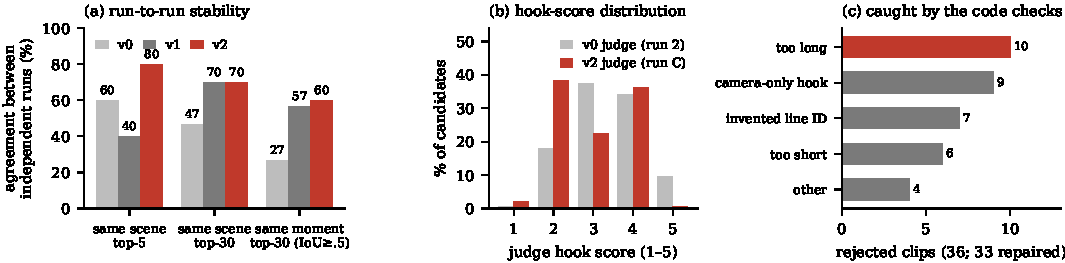
\includegraphics[width=\textwidth]{fig_results.pdf}
\caption{(a) Agreement between two independent runs of each version (v0 first build, v2 final). (b) The early judge
scored almost everything 3--5; after calibration the scores separate clips. (c) Clips rejected by the code checks in
the official run, by reason; 33 of 36 went back to the model with legal fixes.}
\end{figure}

\begin{table}[t]
\begin{minipage}[t]{0.39\textwidth}\vspace{0pt}\small
\captionof{table}{Official run, 50 episodes.}
\begin{tabular}{@{}lr@{}}\toprule
Valid / rejected candidates & 138 / 36\\
Final list & 30 + 2 montages\\
Hard rules re-checked & 32 / 32\\
Clip length, mean & 42\,s (22--59)\\
Blind A/B vs baseline & 13--4 (5 ties)\\
Repeat run, same top-5 scenes & 4 / 5\\
Fast run: calls / time & 103 / 2\,m\,45\,s\\\bottomrule
\end{tabular}
\end{minipage}\hfill
\begin{minipage}[t]{0.575\textwidth}\vspace{0pt}\small
\captionof{table}{Top of the ranked list (screenplay times, computed by code).}
\begin{tabular}{@{}r l >{\raggedright\arraybackslash}p{3.3cm} >{\raggedright\arraybackslash}p{2.6cm}@{}}\toprule
\# & In -- out & Hook & Ends on\\\midrule
1 & E2 00:00--00:45 & ``I cannot marry you, Juliana.'' & ``Do not disgrace us further.''\\
2 & E3 00:58--01:25 & ``Guards! Remove her!'' & ``\dots let her go.''\\
3 & E1 00:11--01:02 & ``You should turn around, Juliana.'' & ``I changed my mind.''\\
4 & E11 00:17--00:51 & ``Your husband stole my gold watch!'' & ``Search it.''\\
5 & E12 00:44--01:25 & ``I want to see you crawl, sister.'' & ``Tell me where the garden is.''\\\midrule
M1 & \multicolumn{3}{@{}>{\raggedright\arraybackslash}p{8.2cm}@{}}{E2 00:00--00:12 + E3 01:06--01:24 + E4 00:50--01:06:
jilted at the altar $\to$ a stranger steps in $\to$ ``It is a vow.''}\\\bottomrule
\end{tabular}
\end{minipage}

\end{table}

\section{Where it picks badly}
\begin{itemize}
\item \textbf{Strict length rule loses moments}: 16 of 36 rejections were too long or short; on the caption test the best
opening line was lost this way.
\item \textbf{Weak endings}: some clips stop on a sad or throwaway line instead of an open question.
\item \textbf{Noise below the top 5}: the same clip's score varies by 0.5--1 point between runs; top-10 agreement is 6/10.
\item \textbf{Blind spots}: visual hooks are read from text; the judge and the picker are the same model family; there is
no human-labelled ground truth, so nothing here proves a clip will perform.
\end{itemize}

\section{Scale}
About 106 model calls per 50-episode show, run in parallel: under 3 minutes instead of 41 (slower on a free key).
A company gateway or stronger models plug in through \texttt{config.yaml}. An editor reviews about 10 ranked clips
instead of watching 50 episodes. The real proof is a live split test of tool- against editor-picked promos on equal
spend, compared on hook rate, hold rate, click-through and cost per install. \textbf{Next:} re-fit the weights from
editor approvals, add audio/visual signals, use a second-family judge, and label a small human gold set.

\section{AI tools used, and where they got it wrong}
Claude Code harness with Qwen models was used in this project; Gemini models run inside the pipeline.
\textbf{Where it went wrong:} asked to fix clips that came out too long or short, Qwen wrote a ``rescue'' that moved
the start and \emph{silently replaced the hook} with whatever line came first. All tests passed; only a manual read of
the picks caught it (the \#1 promo had lost the moment it was chosen for). \textbf{The fix} was a single invariant:
the hook and cliffhanger are pinned anchors, and any repair may only adjust the clip around them. A one-line check
compares the hook text before and after every repair and rejects the clip if it changed, so a silent swap can no
longer reach the output.

\section{Market research: what the ads that run actually look like}
\begin{minipage}[t]{0.36\textwidth}\vspace{0pt}\small
\captionof{table}{Length of the top-impression US video ads in Meta's Ad Library, 8 Nov 2026 (active ads only;
impressions are not installs).}
\begin{tabular}{@{}lrr@{}}\toprule
Ad length & ReelShort & DramaBox\\\midrule
$\le$ 60\,s & 10 & 0\\
1--3 min & 12 & 0\\
3--10 min & 8 & 2\\
$>$ 10 min & 104 (77\%) & 28 (93\%)\\\midrule
Ads sampled & 135 & 30\\\bottomrule
\end{tabular}
\end{minipage}\hfill
\begin{minipage}[t]{0.61\textwidth}\vspace{0pt}
Each finding set a design rule:
\begin{itemize}[leftmargin=1em]
\item \textbf{Long cuts dominate} (Table 3): a pick is also a long ad's cold open, so the 3\,s hook is enforced in code.
\item \textbf{Hidden identity} is the top premise in both apps' ad copy: the title twist sells, it is not a spoiler.
\item \textbf{Conflict opens}: 36\% of long-running drama ads open mid-conflict [AI Vidia]: no camera-only hooks.
\item \textbf{Episode 1 sells}: ReelShort's top creative is from ep.\ 1 [AppGrowing]: early episodes rank higher.
\item \textbf{Volume}: $\sim$1{,}900 creatives per app in H1 2026, fatiguing in 3--5 days [Mobvista, AppGrowing].
\end{itemize}
\end{minipage}
\end{document}
